\documentclass{article}

\begin{document}

To create a data set that enables regression models of the finger kinematics, we need a set of gestures that is as big as possible and allows to distinguish the muscular activity linked to each finger independently even if they do not reflect real life movements. This task is difficult as each gesture involves similar sets of muscles.
The needed gestures are also different than for classification model where the set of gestures only need to be as small as possible and to only contain real life movements.


\subsubsection{Single finger motions}

The simplest set of gesture to estimate simultaneously each finger kinematics is composed only of single finger gestures. That is, flexion and extension of one finger at a time with maximum amplitude. 

This techniques has been used in multiple studies \cite{ref:singleFingerGestPlusSignLang, ref:singleFingerGest1, ref:singleFingerGest2} that tried to create regression and classification model of the finger kinematics. They report to have good prediction accuracy (more than 97.5\% in \cite{ref:singleFingerGestPlusSignLang}) but only share the result of the estimation of single finger gestures. Thus, movements involving more than one fingers might not have a good prediction accuracy.


\subsubsection{Activities of daily living (ADL)}

ADLs are gestures that represents real life movements of everyday life. For example, tying a shoelace or typing on a keypad are considered as ADLs. The advantage of using ADLs as base for an hand gesture regression data set is that they allow to get the mot precision for gestures that the final users will be often performing. The KIN-MUS IJI data set \cite{ref:KinMusUji} based its gestures on 26 ADL. 20 of them are taken from the Sollerman Hand Function test (SHFT), which is often used to evaluate the upper extremity’s functional recovery \cite{doi:SHFT}. These 20 ADL aims at showing similar muscle activation pattern as the eight most common hand grips. Performing ADL gesture involve the subject to interact with objects which must be taken into account for the data collection protocol.


\subsubsection{Sign language}

Studies have tried to create sEMG based devices capable of translating sign language into text \cite{ref:signLang, ref:signLang2}. In particular, the Taiwanese sign language is known to contain 50 fundamental postures which involve lots of linkage of multiple fingers \cite{ref:singleFingerGestPlusSignLang, ref:signLang}.

\begin{figure}[H]
    \centering
    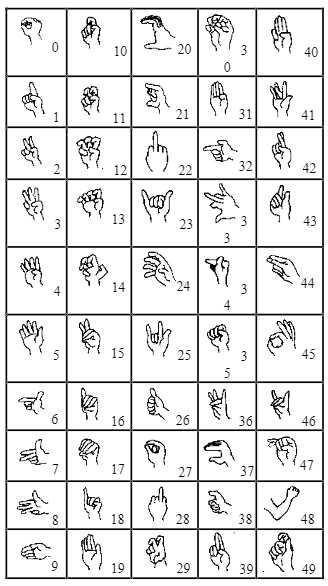
\includegraphics[width=5cm]{images/taiwaneseSignLanguage.png}
    \caption{The 50 fundamental postures of Taiwanese sign language \cite{ref:signLang}}
    \label{fig:signLang}
\end{figure}

Sign languages also has the advantage of giving a set of many postures that are well identifiable from each other. This gives better chance for a classification model to get a high accuracy. It has been shown that, even a small number of sEMG electrodes (organized in a myo armband \cite{ref:myoArmBand}) enable to get classify such gestures with good precision \cite{ref:signLang2}.





\subsubsection{Irregular moves}

A study \cite{ref:Ngeo2014} has used 3 kinds of exercises. The last one was to ask the subject to move its hands freely while keeping a neutral position of the forearm. They encouraged the subject to make irregular gestures in order to get a lot of information on the possible combination of fingers flexion and extension.


\subsubsection{Maximum voluntary contraction (MVC)}

The recording of maximum voluntary contractions allow to find the maximum amplitude of the EMG signals which can be later used to normalize the signals. Normalization of the EMG signal is important because this signal is user dependant. This kind of processing allows to mix results obtained on different subjects in a same data set.
There are height different postures of the hand for which a MVC can be recorded (see figure \ref{fig:mvc}).

\begin{figure}[H]
    \centering
    \includegraphics[width=10cm]{images/mvc.png}
    \caption{Representations of the 8 postures of the hand for which a MVC can be recorded}
    \label{fig:mvc}
\end{figure}

Studies creating synchronized hand kinematics and sEMG data sets have included this kind of recording in their data \cite{ref:Ngeo2014, ref:KinMusUji} but they do not include the 8 possible postures. Their protocol of data collection for MVC was composed of a few records (i.e. 3 records of each MVC) with 3 minutes of resting between each repetition of the set of postures due to the muscle fatigue that it causes, which can lead to less accurate data.

Even if this method of calculating the maximal muscular activity of the forearm is the most widely used in the literature, it does not always give the best results. A study which compared maximum wrist extension with resisted wrist extension \cite{ref:mvc} has shown that using resisting device gives a more accurate measurement of maximal effort.

\end{document}